对应于重要物理量的算符的本征函数,几乎没有例外,都有两个性质:正交性和归一性。
本章的目的是详细地展开这些概念和说明它们的一些应用。 
“展成正交函数”是最重要的概念。
做为这种技巧的举例我们将详细地考察“富里叶级数”。
我们也要学习怎祥用"施密特正交化”造正交函数和怎样从特殊微分方程的解产生正交函数。
为了说明后一概念, 我们将要考察“勒让德多项式”的性质,并简要介绍量子化学中其他重要特殊函数。
在附录中简要地讨论微积分和复变数的基础。
在学习本章前读者最好先检验一下自己对这些内容熟悉的程度。

\section{基本概念:正交性和归一性}
在开始讨论正交函数时,先复习函数概念。
函数概念有三个主要成份。第一,将函数定义在数标上的特殊域内,如从a到b。
第二,存在一变量(如x),它可在a到b域内独立地取值,第三,按特定规则对任意x值都存在确定y值。\footnote{换成我们现在比较熟悉的说法:构造函数这一映射关系需要一个定义完备的定义域和值域以及一个从定义域到值域的映射关系。}
这样,我们可以说在$a \leq x \leq b$域内y是x的函数。
这个定义可用某种方式加以修改以包含多于一个独立变量,但这三个主要成份要保持:一个独立变量;独立变量取值的区间;用一特定规则将因变量与独立变量联系起来。

表述“y是x的函数”的最简单的表示方法是写下方程y=y(x)。
这种表示法很简洁,但可能产生误会。
方程的左端仅是变量的名称——在我们看到方程右端之前并不知它是因变量。
右端也用字母,但这里的符号y( )的含义与单纯变量名称有所不同。
y( )表示y是因变量,它的值可按特定规则由括号里的量求出。
y=y(x)没表示出独立变量x定义的区间。
这在函数概念的初级讨论中并不总是重要的,但在表示函数展开时则是非常重要的。

因此,我们引入一个定义。
\begin{definition}[展开区间或简称区间]
    展开区间是所讨论的函数的独立变量的取值范围。这并不意味着在独立变量取其它值时函数不能定义,只不过不考虑那些别的值。
\end{definition}
   
通常用$[a,b]$表示展开区间,它表示独立变量x允许值在$a \leq x \leq b$范围内。

现在再连续介绍四个定义。
\begin{definition}[内积]
    在展开区间[a,b]内为连续变量的二函数f和g(一般讲是复函数)的内积是:
    \[\bra*{f}\ket*{g}=\int_a^bf(x)^*g(x)\dd{x} \tag{2-1}\]
\end{definition}

二函数的内积是定义在其展开区间内。
有些作者用$(f,g)$表示内积,但这容易和表示維坐标或开城的符号混淆。我们将采
用$\bra*{f}\ket*{g}$。书写的顺序十分重要: 
\[\bra*{g}\ket*{f}=\int g(x)^*f(x)\dd{x}=\left ( \int f(x)^*g(x)\dd{x} \right )^*=\bra*{f}\ket*{g}^* \tag{2-2}\]
对实函数书写顺序不重要。方程2-2说明了以后将反复出现的内积的一个重要特性:对换内积的一函数的位置得出该内积的复共轭。
常数可从内积符号里随意移出:若b和c是(复)数,则$\bra*{bf}\ket*{cg}=b^*c\bra*{f}\ket*{g}$。

内积是一很有意义的概念。它的几何类比是大家可能已熟悉的向量的点积或标量积,我们将在第三章讨论它。

与向量的垂直性这几何性质类比,函数和向量都有正交性这一概括性的和一般化的概念。
\begin{definition}[正交]
    若二函数$f(x)$和$g(x)$在区间$[a,b]$的内积为零,
    \[\bra*{f}\ket*{g}=\int_a^bf^*g=0=\int_a^bg^*f=\bra*{g}\ket*{f} \tag{2-3}\]
    我们就说它们是正交的。
\end{definition}

若内积为零,则内积中哪个函数在前面都行,因此,f和g的正交性既可用$\bra*{f}\ket*{g}=0$表示,也可用$\bra*{f}\ket*{g}=0$表示。
二向量的垂直性可写正交性的这个定义联系起来;若其点积为零,则二向量垂直。

\begin{definition}[范数]
    函数在区间$[a,b]$的范数和自身的内积,可用符号$N$表示:
    \[N(f)=\bra*{f}\ket*{f}=\int_a^bf^*f \tag{2-4}\]
\end{definition}

函数的范数是实的,正量;它与向量的长度的平方类似。
范数是实的正的可证明如下:
\[f^*f=(\text{Re} f-i\text{Im} f)(\text{Re} f+i\text{Im} f)=(\text{Re} f)^2+(\text{Im} f)^2 \tag{2-5}\]
它是正的有限的。于是$f^*f$的积分即范数也是正的有限的。
范数为正值这一性质立刻就有用处。

\begin{definition}[归一性]
    定义若一函数的范数是一,即$\bra*{f}\ket*{f}=1$,则称该函数是归一化\footnote{原书的脚注:归一化为一井非唯一可能的归一化,但它是最常用的,本节始终用它。}的。
\end{definition}

因为函数在特定区间的范教永远是正实数,所以我们总能将一给定函数采一数使之归一化。
假定f的范数是N,那么函数$f/\sqrt{N}$的范数为一,因
\[\bra*{\frac{f}{\sqrt{N}}}\ket*{\frac{f}{\sqrt{N}}}=\frac{1}{N}\bra*{f}\ket*{f}=\frac{N}{N}=1 \tag{2-6}\]

将函数除以它的范数的平方根的过程称为将所数归一化,或有时说将函数归一化为一。

我们将已介绍的五个定义用于些例子。
假定我们讨论的函数定义在区间$[-1,1]$。做为演算内积的例子,我们求算$\bra*{x}\ket*{x^2}$
\[\bra*{x}\ket*{x^2}=\int_{-1}^1x^*x^2\dd{x}=\int_{-1}^1x^3\dd{x}= \eval{\frac{x^4}{4}}_{-1}^1=0 \tag{2-7}\]
此简单内积计算的结果是零。因此,可以讲$x$和$x^2$在$[-1,1]$区间是正交函数。
可看到指定区间的重要性:在$[0,1]$区间内积$\bra*{x}\ket*{x^2}$为
\[\bra*{x}\ket*{x^2}=\int_0^1x^3\dd{x}= \eval{\frac{x^4}{4}}_0^1=\frac{1}{4} \tag{2-8}\]
因而函数不是正交的。必须先指定展开区间,才能讲正交性。对归一性也是这样。
在区间$[-1,1]$函数x的范数为
\[N(x)=\bra*{x}\ket*{x}=\int_{-1}^{1}x^2\dd{x}=\frac{2}{3} \tag{2-9}\]
而在区间$[0,1]$范数为:
\[N(x)=\bra*{x}\ket*{x}=\int_{0}^{1}x^2\dd{x}=\frac{1}{3} \tag{2-10}\]

现在可介绍函数的一个非常有用的性质。
形成内积的积分常常可用函数的对称性来简化。
用两个定义表示对称性。

\begin{definition}[奇偶性]
    定义若$f(x)=f(-x)$,则函数是偶函数; \\
    若$f(x)=-f(-x)$,则函数是奇函数。
\end{definition}

偶或奇很容易用图表示出。图2-1$a$示出函数$f(x)=x^2$的图:因$(x)^2=(-x)^2$,所以它是偶函数。
按图形讲,f(x)的图形对纵坐标对称。
图2-1b示出函数$f(x)=x^3$的图, 因$(x)^3=-(-x)^3$,所以它是奇函数。
图在纵坐标右边的部分是左边部分的负值。
若区间对称,则偶或奇函数的积分特别简单。可归结为下列定理。

\begin{figure}[htbp]
    \centering
    \begin{minipage}[t]{0.48\textwidth}
    \centering
    \includegraphics[width=6cm]{./fig/2-1a.png}
    
    (a)
    \end{minipage}
    \begin{minipage}[t]{0.48\textwidth}
    \centering
    \includegraphics[width=6cm]{./fig/2-1b.png}
    
    (b)
    \end{minipage}
    \caption{偶函数和奇函数}
    \end{figure}

\begin{theorem}
    偶函数在对称区间的积分是在半区间的积分的两倍; \\
    奇函数在对称区间的积分为零。
\end{theorem}

\begin{figure}[htbp]
    \centering
    \begin{minipage}[t]{0.6\textwidth}
    \centering
    \includegraphics[width=6cm]{./fig/2-2a.png}
    
    (a)偶函数在对称区间的积分为半区间的积分的两倍
    \end{minipage}
    \begin{minipage}[t]{0.6\textwidth}
    \centering
    \includegraphics[width=6cm]{./fig/2-2b.png}
    
    (b)奇函数在对称区间的积分为零
    \end{minipage}
    \caption{偶函数和奇函数的积分}
\end{figure}

图2-2示出该定理的图解。可用将整个区间分为二半区间的办法证明:
\[\int_{-a}^a(even)=\int_{-a}^0(even)+\int_0^a(even) \tag{2-11}\]
但因x的偶函数和一x的偶函数一样,所以可用在正半区间$[0,a]$的积分替换在负半区间$[-a,0]$的积分而函数不变:
\[\int_{-a}^a(even)=\int_{-a}^0(even)+\int_0^a(even)=2\int_0^a(even) \tag{2-12}\]
这就证明了定理的第一部分。第二部分的证明也同样简单:
\[\int_{-a}^a(odd)=\int_{-a}^0(odd)+\int_0^a(odd)=-\int_0^a(odd)+\int_0^a(odd)=0 \tag{2-13}\]
奇函数在负半区间的积分可用在正半区间的积分的负值替换。方程2-13给出定理的第二部分。

将此定理应用于对称区间的内积得到另一结果。
\begin{theorem}
    在对称区间$[-a,a]$,奇函數与奇函数或偶函数与偶函数的内积不为零,并可由在半区间$[-a,0]$或$[0,a]$的内积的二倍算出;不论函数是什么形式,偶函数与奇函数的内积为零。
\end{theorem}

在上述五个定义里,我们只考虑了二任意函数。但这些定义的威力和有效性对于函数组无疑也是很明显的。
函数组是函数的集合,它们的变量相同,定义区间相同,和写出函数的规则相同。
例如,x的全部幂函数构成一组函数。
这个函数组用大括号可写
成$\{x^n\}$,它表示这些x的函数的全部:$x^0=1$,$x^1=x$,$x^2$,$x^3$,$x^4$等等。
一般项的指数n表明写出函数组中每个成员的规则。
为了完备起见,必须标明区间和n (常称为指标)可取的值,如下边那样:
“函数组$\{x^n\}$,在$[-1,1]$,$n=0$和全部正整数”。

为了完善地描述量子化学中有用的函数组,我们引人三个新定义。

\begin{definition}[完备函数集]
    完备函数组$\{F_i\}$是这样的函数组,任何别的函数$f$都可在规定的展开区间用函数组$\{F_i\}$的成员线性组合表示,并可达到你所要求的任何精确度
    \footnote{原书的脚注:在这里和以后都默认函数组$\{F_i\}$和函数$f$是均匀连续的,若用了这个概念,则该定义可更严格些,但这在量子化学中是不重要的。}。
\end{definition}

若函数组$\{F_i\}$是完备的,则$f$可展成函数$F_i$.如下:
\[f(x)=a_1F_1(x)+a_2F_2(x)+ \cdots +a_nF_n(x)+ \cdots =\sum_{n=1}^{+\infty}a_nF_n(x) \tag{2-14}\]
一般讲,要证明一函数组是否完备是十分困难的,但根据我们的目的要求,将只考虑已知它们是完备的那些函数组,而不考虑完备性的证明本身。

\begin{definition}[正交完备函数集]
    一函数正交组或正交函数组是这样的函数组,在规定的区间内其中每一函数与全部其它函数都是正交的。
\end{definition}

即若函数组$\{F_i\}$中每一成员与每一其它成员正交,
\[\bra*{F_j}\ket*{F_k}=0 \tag{2-15}\]
对全部j和k$(j \neq k)$,是正交组。
在本章第三节要讨论的函
数组$\{\sin nx,\cos nx\}$在区间$[-\pi,\pi]$,$n=0$或正整数,就是这样的函数组。
证明这些函数组的正交性是本章未要讨论的问题之一;请注意它是三个分开的证明\footnote{作者这里可能想表达三角函数系正交性的三种体现可以分别证明,但对2-16c个人认为改为$\bra*{\sin nx}\ket*{\cos mx}=0 \quad for \ all$ \\ $ \ n,m$更合适,按照原文表述并未完全体现三角函数系的正交性的涵义。}:
\[
\begin{array}{rl}
    \bra*{\sin nx}\ket*{\sin mx}=0 & n \neq m \\
    \bra*{\cos nx}\ket*{\cos mx}=0 & n \neq m \\
    \bra*{\sin nx}\ket*{\cos nx}=0 & for \ all \ n
\end{array}    
\tag{2-16}
\]

最后,将正交性和归性合并在一起。

\begin{definition}[正交归一完备函数集]
    定义正交归一函数组是函数的正交组,其中每一函数又是归一化的。
\end{definition}

即若
\[\bra*{F_j}\ket*{F_k}=0, \ \text{for all} \ j \neq k \tag{2-17a}\]
\[\bra*{F_j}\ket*{F_j}=0, \ \text{for all} \ j=k \tag{2-17b}\]
则$\{F_i\}$是正交归一的。
在讨论正交归一函数时2-17a和2-17b这一对方程要经常出现,因此需要引入一特殊符号将方程2-17a和方程2-17b合并在一起。
克朗尼克符号($\delta_{ij}$)的含义是当$i \neq j$,$\delta_{ij}=0$;当$i=j$,$\delta_{ij}=1$。
若用克朗尼克符号,则正交归一的条件(方程2-17a和方程2-17 b)可简单地表示为
\[\bra*{F_j}\ket*{F_k}=\delta_{ij}, \ \text{for all} \ j,k \tag{2-18}\]
在本章中正交归一组是用小写希腊字母表示,如$\{\phi_i\}$。
在本节中我们定义了一些重要术语,内积,正交性,范数和归一性,完备性,正交和正交归一函数组;我们也应用函数的偶和奇性质简化在对称区间的积分。

\section{用正交归一函数组展开}
在本节中,我们将要学习如何在规定区间将给定函数用一组正交归一函数展开。
因这种演算过程在接着讨论正交归一函数和以后讨论正交归一向量时经常出现,所以先将这些计算公式写出。
\[f(x)=\sum_ia_i\phi_i(x) \tag{2-19}\]
\[\phi_j(x)^*f(x)=\sum_ia_i\phi_j(x)^*\phi_i(x) \tag{2-20}\]
\[\int\phi_j(x)^*f(x)\dd{x}=\sum_ia_i\int\phi_j(x)^*\phi_i(x)\dd{x} \tag{2-21}\]
\[\bra*{\phi_j}\ket*{f}=\sum_ia_i\bra*{\phi_j}\ket*{\phi_i} \tag{2-22}\]
\[\bra*{\phi_j}\ket*{f}=\sum_ia_i\delta_{ji} \tag{2-23}\]
\[\bra*{\phi_j}\ket*{f}=a_j \tag{2-24}\]

方程2- 19表示$f(x)$在特定展开区间(这里未标明)展成正交归一函数组$\{\phi_i\}$的成员的线性组合。
方程2-20是将方程2-19的两端都乘以函数组$\{\phi_i\}$中的任一函数的复共轭$\phi_i(x)^*$的结果。
方程2-21是将方程2- 20的两端在展开区间积分的结果。
而方程2-20和2 21就是$\phi_j$(在左)与方程2-19 (在右)形成的内积。

在方程2-23中根据正交归一的定义以克朗尼克符号$\delta_{ji}$代替$\bra*{\phi_j}\ket*{\phi_i}$。

最后,对方程2-23的右端求和。若将求和写出,则其形式如下:
\[\sum_ia_i\delta_{ji}=a_1\delta_{j1}+a_2\delta_{j2}+ \cdots +a_j\delta_{jj}+ \cdots +a_n\delta_{jn}+ \cdots \tag{2-25}\]

除一个克朗尼克符号外其余的皆为零。仅有的一个不为零的克朗尼克符号是$\delta_{jj}=1$。于是求和给出
\[\sum_ia_i\delta_{ji}=a_j\delta_{jj}=a_j \cdot 1=a_j \tag{2-26}\]

使用在正交归一性基础上产生的克朗尼克符号是在展成正交归一函数时,简化求算系数$a_i$的关键。
方程2-23中的求和遵守一简单的规则:在对包含克朗尼克符号和别的量的乘积求和时,只挑选出包含下标相同的克朗尼克符号的项就行,或只剩下包含下标相同的克朗尼克符号的项。

最后,方程2-24是在给定区间将一函数展成正交归一函数组的展开系数的计算公式,$a_j=\bra*{\phi_j}\ket*{f}$。展开系数可以是复数。
不要用错下标!若需要$a_1$,就要求算$\bra*{\phi_1}\ket*{f}$,需要$a_2$,就求算$\bra*{\phi_2}\ket*{f}$;需要$a_3$,就求算$\bra*{\phi_3}\ket*{f}$,以此类推。下节我们将详细地举一例。

下边我们转入一在实用上重要的问题。若将展成正交归一组的展开式中若干项后各项断掉,产生的误差是多少?
在回答此问题中显现出展开系数的一个新性质:这些系数可使断尾展开式的误差极小。用$M_n$表示取n项的误差。此误差可用下式求出\footnote{原书的脚注:这是误差的“最小二乘法”判别。别的方法也可以用。还应注意,如果整个函数是归一化的,则断尾展开式不是归一化的。};
\[M_n=\int\abs\Big{f(x)-\sum_{j=1}^nb_j\phi_j}^2\dd{x} \tag{2-27}\]

即,用余项的绝对值的平方与x对划的曲线下的面积求算。
积分范围是展开区间。在图2-3中用图说明$M_n$的含义。因$c^*c=\abs*{c}^2$,故可写成
\[M_n=\int \left ( f^*-\sum_{j=1}^nb_j^*\phi_j^* \right ) \left ( f-\sum_{i=1}^nb_j\phi_j \right )\dd{x}\]
\[=\bra*{f}\ket*{f}-\sum_{j=1}^nb^*_j\bra*{\phi_j}\ket*{f}-\sum_{i=1}^nb_j\bra*{f}\ket*{\phi_j}+\sum_{j=1}^n\sum_{i=1}^nb_j^*b_i\bra*{\phi_j}\ket*{\phi_i} \tag{2-28}\]

注意方程2-28中每个因式所用的求和指标不同。求和指标常常只是傀标,因为它们的名称单独存在并无什么特殊意义。然而,对它们的名称却必须时常小心地加以辨别。例如,
\[\left (\sum_ic_i\phi_i\right )\left (\sum_ic_i\phi_i\right )\]
可能误写为
\[\sum_ic_i^2\phi_i^2\]
\begin{figure}[htbp]
    \centering
    \includegraphics[scale=0.6]{./fig/2-3.png}
    \caption{展成正交归一函数的断尾展开的误差}
\end{figure}
但它不是乘积的含义。若加和写出,$(c_1\phi_1+c_2\phi_2+ \cdots )(c_1\phi_1+c_2\phi_2+ \cdots )$等于$c_1^2\phi_1^2+c_1c_2\phi_1\phi_2+c_2c_1\phi_2\phi_1+c_2^2\phi_2^2 \cdots $,它与
\[\sum_ic_i^2\phi_i^2=c_1^2\phi_1^2+c_2^2\phi_2^2+ \cdots\]
差别很大。为了保证写出的答案正确(包含交错项),我们使用下列符号
\[\left (\sum_ic_i\phi_i\right )\left (\sum_jc_j\phi_j\right )=\sum_{ij}c_ic_j\phi_i\phi_j\]

因函数组$\{\phi_i\}$是正交归一的,所以方程2-28的末项中可代入克朗尼克符号\footnote{原书合并后最后一项连加的符号误写为+。}:
\[M_n=\bra*{f}\ket*{f}-\sum_{j=1}^nb^*_j\bra*{\phi_j}\ket*{f}-\sum_{i=1}^nb_j\bra*{f}\ket*{\phi_j}+\sum_{j=1}^n\sum_{i=1}^nb_j^*b_i\delta_{ij}\]
\[=\bra*{f}\ket*{f}-\sum_{j=1}^n \left ( b^*_j\bra*{\phi_j}\ket*{f}+b_j\bra*{f}\ket*{\phi_j}-b_j^*b_j \right ) \tag{2-29}\]

在包含克朗尼克符号的项中对$i$求和,只剩下$i=j$的项,又因求和指标的名称不重要,故三项都用指标$j$表示,并且并在一起。

我们可借助使与系数$b_j$对应的误差$M_n$极小的办法求展开系数的“最佳”组。
因为$b_j$,有实数和虚数两部分,所以它包含两步。
双极小问题可表为对全部$j$求$\partial M_n / \partial b_j=\partial M_n / \partial b_j^*=0$。
对方程2-29求导数得出
\[\frac{\partial M_n}{\partial b_j}=0=-\bra*{f}\ket*{\phi_j}+b^*_j \tag{2-30a}\]
\[\frac{\partial M_n}{\partial b_j^*}=0=-\bra*{\phi_j}\ket*{f}+b_j \tag{2-30b}\]
这两个方程彼此成复共轭,从使误差为极小的意义看,展开式的“最佳”系数可由下式求出:
\[b_j=\bra*{\phi_j}\ket*{f} \tag{2-31}\]
由方程2-31得出的系数事实上就是展成正交归一函数时必须使用的系数。
因此,$a_j=b_j=\bra*{\phi_j}\ket*{f}$\footnote{这里莫名其妙的换了系数的符号我猜是作者同时参考了两本书发现符号不同但是懒得改了(笑)。}不仅是 “正确”的系数(方程2-24),而且也是“最佳”的系数(方程2-31)。

将$a_j=b_j=\bra*{\phi_j}\ket*{f}$代入方程2-29,求出的误差为
\[M_n=\bra*{f}\ket*{f}-\sum_{j=1}^n \left ( a_ja_j^*+a_j^*a_j-a_j^*a_j \right )=\bra*{f}\ket*{f}-\sum_{j=1}^n\abs*{a_j}^2 \tag{2-32}\]

我们用一个称为展开定理的有关内积的重要关系结束本节。

\begin{theorem}
    内积$\bra*{f}\ket*{g}$可 用正交归一函数组$\{\phi_i\}$展开为
    \[\bra*{f}\ket*{g}=\sum_i\bra*{f}\ket*{\phi_i}\bra*{\phi_i}\ket*{g} \tag{2-33}\]
\end{theorem}

为了证明此定理,可将$f$展成$f=\sum_ia_i\phi_i$,$g$展成$g=\sum_ib_i\phi_i$。于是
\[\bra*{f}\ket*{g}=\int f^*g=\sum_i\sum_j\int a^*_i\phi_J^*b_j\phi_j=\sum_{ij}a_i^*b_j\bra*{\phi_i}\ket*{\phi_j}=\sum_{ij}a_i^*b_j\delta_{ij}\]
而
\[a_i^*=\bra*{\phi_i}\ket*{f}^*=\bra*{f}\ket*{\phi_i},b_i=\bra*{\phi_i}\ket*{g}\]
因此,
\[\bra*{f}\ket*{g}=\sum_i\bra*{f}\ket*{\phi_i}\bra*{\phi_i}\ket*{g}\]

展开定理中出现的结构$\ket*{\phi_i}\bra*{\phi_i}$在本书后边将赋予更多的含义。
现在我们在展开定理中看到的只是在$\bra*{f}$和$\ket*{g}$之间插入$\ket*{\phi_i}\bra*{\phi_i}$对$i$求和。
这就是实际情况;这种运算称为“插入态的完备组”。
展开定理可写成$\sum\ket*{\phi_i}\bra*{\phi_i}=1$。
结构$\ket*{\phi_i}\bra*{\phi_i}$不是方程2-29定义的内积,它是我们到此为止还未讨论的一个元素。
它实际上是一个算符。以后会明显地看到它起着算符的作用。

在本节中,我们导出了展成正交归一函数组的展开式中系数公式;证明了这些系数使断尾展开式的误差极小,并导出断掉展开式\footnote{我觉得叫断尾展开式或者截尾展开式都比这个好。}的余项产生的误差公式。最后,导出内积的展开定理。

\section{富里叶(Fourier)级数}

富里叶级数\footnote{古早翻译了属于是。}是将函数展成与${\sin mx,\cos \, mx}$成比例的正交归一函数组的展开式。
在第一节中讲过这些函数是正交的,现在导出它在$[-\pi,\pi]$区间的范数。
\[N(\sin mx)=\bra*{\sin mx}\ket*{\sin mx}=\int_{-\pi}^{\pi}\sin^2 \, mx\dd{x}=\frac{1}{m}\int_{-m\pi}^{m\pi}\sin^2y\dd{y}=\pi \tag{2-34}\]
同样
\[N(\cos mx)=\bra*{\cos mx}\ket*{\cos mx}=\int_{-\pi}^{\pi}\cos ^2 \, mx\dd{x}=\frac{1}{m}\int_{-m\pi}^{m\pi}\cos ^2y\dd{y}=\pi \tag{2-35}\]
方程2-34和2-35除m=0外对全部m值都成立,而m=0时则得出不定的N=0/0。为了澄清m=0的情况,必须分开求算
\[N(\sin \, 0x)=\bra*{\sin \, 0x}\ket*{\sin \, 0x}=\int_{-\pi}^{\pi}0\dd{x}=0 \tag{2-36}\]
\[N(\cos  \, 0x)=\bra*{\cos  \, 0x}\ket*{\cos  \, 0x}=\int_{-\pi}^{\pi}1\dd{x}=2\pi \tag{2-37}\]
全部结果可以表为
\[
N(\sin mx)=\left\{
\begin{array}{rl}
    \pi, & m \neq 0 \\
    0, & m=0
\end{array}
\right.
\qquad
N(\cos mx)=\left\{
\begin{array}{rl}
    \pi, & m \neq 0 \\
    2\pi, & m=0 \\
\end{array}  
\right.  
\tag{2-38a}
\]
或用克朗尼克符号表示
\[
\begin{array}{c}
    N(\sin mx)=\pi-\pi \delta_{m0} \\
    N(\cos mx)=\pi+\pi \delta_{m0}
\end{array}    
\tag{2-38b}
\]
与正交关系式合在一起,可写出$(\sin mx ,\cos mx)$的全部可能的内积
\[
\begin{array}{c}
    \bra*{\sin mx}\ket*{\cos mx}=0 \\
    \bra*{\sin mx}\ket*{\sin nx}=(1-\delta_{m0})\pi \delta_{mn} \\
    \bra*{\cos mx}\ket*{\cos nx}=(1+\delta_{m0})\pi \delta_{mn}
\end{array}    
\tag{2-39}
\]

对全部m,n为任意正整數或零。因为我们要用以前的公式(方程2-24)来计算展成正交归一函数组的展开系数,所以必须用函数组
$\{(2\pi)^{-\frac{1}{2}},(\pi)^{-\frac{1}{2}}\sin mx,(\pi)^{-\frac{1}{2}}\cos mx\}$, $m=1,2,\cdots $,$[-\pi,\pi]$代替函数组${\sin mx ,\cos mx}$。

对于这些正交归一函数,展开系数为
\[
\begin{array}{c}
    a_0=\bra*{\frac{1}{\sqrt{2\pi}}}\ket*{f} \\
    a_m=\bra*{\frac{\cos mx}{\sqrt{\pi}}}\ket*{f} \\
    b_m=\bra*{\frac{\sin mx}{\sqrt{\pi}}}\ket*{f}
\end{array}    
\tag{2-40}
\]
展开式为
\[f(x)=\frac{a_0}{\sqrt{2\pi}}+\sum_{m=1}^{+\infty}\frac{a_m}{\sqrt{\pi}}\cos mx+\sum_{m=1}^{+\infty}\frac{b_m}{\sqrt{\pi}}\sin mx \tag{2-41}\]
这不是富里叶级数的一般形式,只是展成正交归一函数组的一个例子。一般是利用以显式写出展开系数的办法将常数移到项外:
\[f(x)=\frac{\bra*{1}\ket*{f}}{2\pi}+\frac{1}{\pi}\sum_{m=1}^{+\infty}(\bra*{\cos mx}\ket*{f}\cos mx+\bra*{\sin mx}\ket*{f}\sin mx) \tag{2-42}\]
最终的结果是
\[f(x)=\frac{c_0}{2}+\sum_{m=1}^{+\infty}c_m\cos mx+\sum_{m=1}^{+\infty}d_m\sin mx \tag{2-43}\]
\[c_m=\frac{1}{\pi}\bra*{\cos mx}\ket*{f} \tag{2-44a}\]
\[d_m=\frac{1}{\pi}\bra*{\sin mx}\ket*{f} \tag{2-44b}\]
在$[-\pi,\pi]$区间。这是富里叶级数常用的形式。注意首项被2除。
这是因为$\cos  \, 0x$的范数是2π,对其它全部m值,$\cos mx$的范数是π。

我们能用偶函数和奇函数的性质立刻做出富里叶级数的两个简单推论。
正弦函数是奇函数:$\sin\, x=-\sin(-x)$。余弦函数是偶函数:$\cos  \, x=\cos (-x)$。因此,我们可以写出两个规则。

(1)一奇函数在$[-\pi,\pi]$区间的富里叶展开仅由正弦项组成:$f(x)=\sum d_m\sin mx$。
(1)一偶函数在$[-\pi,\pi]$区间的富里叶展开仅由余弦项组成:$f(x)=\sum c_m\cos mx$。
因为若f是奇函数,则所有内积$\bra*{\cos mx}\ket*{f}=0$;
若f是偶函数,则所有内积$\bra*{\sin mx}\ket*{f}=0$。
例

$f(x)=x$在$[-\pi,\pi]$的展开。因$f(x)=x$是奇函数,所以仅正弦项存在,因此可写成
\[x=\sum_{m=1}^{+\infty}d_m\sin mx, \ m=1,2, \cdots \ in \ [-\pi,\pi]\]
式中
\[d_m=\frac{1}{\pi}\bra*{\sin mx}\ket*{x}=\frac{1}{\pi}\int_{-\pi}^{\pi}x\sin \,mx\dd{x}=\frac{1}{m^2\pi}\int_{-m\pi}^{m\pi}y\sin y\dd{y}=\eval{\frac{1}{m^2\pi}(-y\cos y+\sin y)}_{-m\pi}^{m\pi}\]
\[=-\frac{m\pi \cos  \, m\pi+m\pi \cos  \,m\pi}{m^2\pi}=\frac{2(-1)^{m+1}}{m}\]
富里叶级数为
\[x=\sum_{m=1}^{+\infty}\frac{2(-1)^{m+1}}{m}\sin mx=2\sin \, x-\sin \, 2x +\frac{2}{3}\sin \, 3x -\cdots\]

三项后断尾的富里叶级数和函数本身的比较示于图2-4。可利用方程2-32求出取三项的富里叶级数的均方误差如下:
\[M_3=\bra*{x}\ket*{x}-\sum_{j=1}^3\abs*{a_j}^2 \tag{2-45}\]
根据方程2-40和2-44,$a_j=\sqrt{\pi}d_j$,可得
\[M_3=\int_{-\pi}^{\pi}x^2\dd{x}-4\pi-1\pi-\frac{4}{9}\pi=\frac{2\pi^3}{3}-\frac{49\pi}{9} \approx 6.8\]
其平方根为2.6,可与函数下的面积$\pi^2=9.9$比较。因此,断掉三项后的余项造成的相对误差约为26\%。

\begin{figure}[htbp]
    \centering
    \includegraphics[scale=0.4]{./fig/2-4.png}
    \caption{在区间$[-\pi,\pi]$的函数$f(x)=x$及其富里叶级数展开(A)一项,(B)两项,(C)三项}
\end{figure}

用富里叶级数描述函数有一重要的电子学类比。在通常情况下,很容易在电路中发生正弦和余弦函数。
也可用电子学中的富里叶合成发生其它函数。用这种合成可发生如图2-5a所示的所谓“锯齿”波。
锯齿波是在$[-\pi,\pi]$区间无穷级数$f(x)=x$与对划得到的图,它具有前例中导出的富里叶组分。
图2-5b表示锯齿波的三项近似图。这样的波形被用于示波器和电视中扫描。

\begin{figure}[htbp]
    \centering
    \begin{minipage}[t]{0.7\textwidth}
    \centering
    \includegraphics[width=8cm]{./fig/2-5a.png}
    
    (a)
    \end{minipage}
    \begin{minipage}[t]{0.7\textwidth}
    \centering
    \includegraphics[width=8cm]{./fig/2-5b.png}
    
    (b)
    \end{minipage}
    \caption{(a)“锯齿”波 \quad (b)锯齿波的三项富里叶合成}
\end{figure}

函数$\{\sin mx\}$和$\{\cos mx\}$无论在半区间$[-\pi,0]$或$[0,\pi]$中都是完备的。
这些函数在哪个半区间也都是正交的。
除$\cos  \, 0x$的范数是$\pi$外,所有其它函数的范数都是$\frac{\pi}{2}$因此,我们能够造两个不同的“半富里叶级数”:
\[f(x)=\frac{c_0}{2}+\sum_{m=1}^{+\infty}c_m\cos mx \qquad c_m=\frac{2}{\pi}\bra*{\cos mx}\ket*{f} \tag{2-46}\]
\[f(x)=\sum_{m=1}^{+\infty}d_m\sin mx \qquad d_m=\frac{2}{\pi}\bra*{\sin mx}\ket*{f} \tag{2-47}\]
它们的展开区间都是$[-\pi,0]$或$[0,\pi]$。
无论全富里叶级数还是半富里叶级数都可用按比例展开的办法推广到任何对称区间
$[-a,a]$或半对称区间$[-a,0]$或$[0,a]$,如
\[f(x)=\frac{c_0}{2}+\sum_{m=1}^{+\infty} \left ( c_m\cos \frac{m\pi x}{a}+d_m\sin\frac{m\pi x}{a} \right ) \tag{2-48}\]
\[c_m=\frac{1}{a}\bra*{\cos \frac{m\pi x}{a}}\ket*{f} \qquad d_m=\frac{1}{a}\bra*{\sin\frac{m\pi x}{a}}\ket*{f}\]
在量子力学中富里叶级数的一个重要的经过修正的形式为\footnote{这个形式的强大之处在于它是复数域的傅里叶变换,但一般量子化学不太涉及复变函数的运算,以至于大部分人直接只把它认成一般实数域下的傅里叶变换的简洁形式。}
\[f(x)=\sum_{m=-\infty}^{+\infty}a_me^{imx} \qquad x \in [-\pi,\pi] \tag{2-49}\]
因为若$\{\sin mx,\cos mx\}$对全部正m值和零是完备的,则${e^{imx}=\cos mx + i\sin mx}$对m的全部整数值(正,负和零)也是完备的。
可将函数组$\{e^{imx}\}$的复共轭包括在内,以使函数组完备。
基本富里叶级数的这些修正形式是本章末许多问题中要讨论的课题。

本节展示了非常有用的正交归一函数组展开,富里叶级数(展成正弦和余弦函数),并对它的用途和适用范围做了评论。

\section{构造正交归一函数}
到目前为止我们已一般地讨论了正交归一函数组的性质,它们在级数展开中的应用,以及富里叶级数这个特殊例子。
我们曾经指出,无论正交归一否,唯有函数组是完备的才能得到足够精确的展开。
本节将介绍如何由一完备函数组形成完备正交归函数组。
在实际造完备正交归一函数前,必须引入与完备性有关的一个问题,此问题在目前的讨论和紧接着的工作中都起着重要作用。
我们从一个定义开始。

\begin{definition}[线性无关,线性相关]
    若一函数组中任一函数都不能用其余函数的线性组合来表示,则称该函数组为线性无关的。同样的,若至少有一函数可以线性方程与一个或多个其它函数关联,则称该函数组为线性相关的。
 \end{definition}
此定义可用数学公式表示为,若方程
\[\sum_iC_iF_i=C_1F_1+C_2F_2+ \cdots \tag{2-50}\]
仅当所有的$C_i=0$时才可解,则函数组$\{F_i\}$是线性无关的。若该方程在至少有一个$C_i \neq 0$时可解,则$\{F_i\}$是线性相关的。取下列两组函数为例:
\[
\begin{array}{ll}
    F_1=1 & G_1=1 \\
    F_2=x & G_2=x \\
    F_3=7x+4 & G_3=x^3 \\
    F_4=x^3 & G_4=x^3
\end{array}    
\]
函数组$\{G_i\}$是线性无关的。不可能使这些函数的任何线性组合如方程2-50那样为零。
另一种说法是,这四个函数没有线性关系:$G_3=x^2$不是$1$, $x$和$x^3$的线性组合。$\{F_i\}$是线性相关的。$F_3$是$F_1$,$F_2$和$F_4$的线性组合;$F_3=7F_2+4F_1$。
即方程2-50可在有些$C_i \neq 0$时解出;$-4F_1-7F_2+1F_3+0F_4=0$。

一完备函数组总是包含一线性无关子集(亚组)。这是我们未做证明的一个重要表述;它是造完备正交归一函数组的第一步。

我们用在$[-1,1]$区间x的幂函数为例。泰勒定理从根本上保证函数组$\{x^n\}$,$n=0,1,2 \cdots $,是完备的。
我们也已看到这些函数是线性无关的。再看下列函数组。$\{F'_i\}$是完备的;可从$\{F'_i\}$中将线性相关的组分移出而形成线性无关的函数组$\{F_i\}$。
$\{G_i\}$也是线性无关的和完备的;它与$\{F_i\}$的差别仅仅是排列次序不同。

\[
\begin{array}{ccc}
    \{F'_i\} & \{F_i\} & \{G_i\} \\
    1 & 1 & 1 \\
    x & x & x^2 \\
    2x & \cdots & x^4 \\
    x^2 & x^2 & \cdots \\
    x^3 & x^3 & x \\
    x^4 & x^4 & x^3 \\
    \cdots & \cdots & \cdots
\end{array}    
\]

总是可以从一完备的线性无关的函数组造一完备的正交归一函数组。造正交归一函数组的方法称为施密特正交化。
我们不准备对该方法作全面介绍,只想讲清楚概念,叙述一般结论,然后举一例说明之。
假定有一定义在特定区间的完备的,线性无关的函数组$\{f_i\}$。我们希望用$\{f_i\}$造一正交归一函数组$\{\phi_i\}$。

第一步,令$\phi_0$为归一化的$f_0$。即,使第一个$\phi$函数只与第一个$f$函数成比例。
$f_0$的范数是$N_0=\bra*{f_0}\ket*{f_0}$,因此,$\phi_0=f_0/\sqrt{N_0}$。

第二步,令$\phi_1$为$\phi_0$和$f_1$的线性组合,它与$\phi_0$正交,且是归一化的。 
因$\{f_i\}$是线性无关的所以一般讲这是办的到的。即,
\[\phi_1=\frac{1}{\sqrt{N_1}}(c\phi_0+f_1) \tag{2-50}\]
\[\bra*{\phi_0}\ket*{\phi_1}=0 \tag{2-51}\]
正交条件给出
\[c\bra*{\phi_0}\ket*{\phi_0}+\bra*{\phi_0}\ket*{f_1}=0 \tag{2-53a}\]
\[c=-\bra*{\phi_0}\ket*{f} \tag{2-53b}\]
于是,
\[\phi_1=\frac{1}{\sqrt{N_1}}(f_1-\bra*{\phi_0}\ket*{f_1}\phi_0) \tag{2-54}\]
和
\[N_1=\bra*{f_1}\ket*{f_1}-\bra*{\phi_0}\ket*{f_1}\bra*{f_1}\ket*{\phi_0}-\bra*{\phi_0}\ket*{f_1}\bra*{\phi_0}\ket*{f_1}+\bra*{\phi_0}\ket*{f_1}^2=\bra*{f_1}\ket*{f_1}-\abs*{\bra*{\phi_0}\ket*{f_1}}^2 \tag{2-55}\]

这种步骤一直继续到完备的正交归一函数组造好为止。一般项为
\[\phi_k=\frac{1}{\sqrt{N_k}} \left ( f_k-\sum_{j=0}^{k-1}\bra*{\phi_j}\ket*{f_k}\phi_j \right ) \tag{2-56}\]
\[N_k=\bra*{f_k}\ket*{f_k}-\sum_{j=0}^{k-1}\abs*{\bra*{\phi_j}\ket*{f_k}}^2 \tag{2-57}\]

从讨论中应该搞清楚,如果函数的范数不是有限值,则这些函数就不能归一化。
并非所有函数在所有区间内都是可归一化的;如,函数组$\{x^n\}$在$[-\infty,\infty]$就不是可归一化的。
分子结构的量子力学涉及的函数组几乎都是可归一化的,或平方可积的。

取在全区间$[-\infty,\infty]$函数组$\{x^ne^{-\frac{1}{2}x^2}\}$\footnote{原书中这个函数集的形式写成了$\{e^{-\frac{1}{2}x^2}x^n\}$,我觉得不好看所以给他换过来了。}做为施密特正交化的例子。先证明这些函数是可归一化的。
\[\bra*{f_n}\ket*{f_n}=\int_{-\infty}^{+\infty}e^{-\frac{1}{2}x^2}x^ne^{-\frac{1}{2}x^2}x^n\dd{x}=\int_{-\infty}^{+\infty}e^{-x^2}x^{2n}\dd{x} \tag{2-58}\]
因为被积函数是偶函数,故可使积分简化为
\[\bra*{f_n}\ket*{f_n}=2\int_{0}^{+\infty}e^{-x^2}x^{2n}\dd{x}=\int_{0}^{+\infty}e^{-y}y^{n-\frac{1}{2}}\dd{y} \tag{2-59}\]
用部分积分连续积分给出
\[\bra*{f_n}\ket*{f_n}=\left ( n-\frac{1}{2} \right )\left ( n-\frac{3}{2} \right ) \cdots \left ( \frac{1}{2} \right )\int_{0}^{+\infty}e^{-y}y^{-\frac{1}{2}}\dd{y}\]
\[=2\left ( n-\frac{1}{2} \right )\left ( n-\frac{3}{2} \right ) \cdots \left ( \frac{1}{2} \right )\int_{0}^{+\infty}e^{-x^2}\dd{x}\]
\[=(2n-1)(2n-3) \cdots (3)(1)\frac{\sqrt{\pi}}{2^n} \tag{2-60}\]
式中是将已知积分$\int_0^{+\infty}e^{-x^2}\dd{x}=\frac{\sqrt{\pi}}{2}$代入。对所有的n,范数$N_n$都是有限值。
因此$\{e^{-\frac{1}{2}x^2}x^n\}$中所有函数都是可归一化的。
衰减指数函数$e^{-\frac{1}{2}x^2}$的存在使积分是有限的和函数是平方可积的。

要造正交归一函数组,先将$f_0=e^{-\frac{1}{2}x^2}x^0=e^{-\frac{1}{2}x^2}$归化。
其范数为$\sqrt{\pi}$,故得到$\phi_0=\pi^{-\frac{1}{4}}e^{-\frac{1}{2}x^2}$。
用方程2-54和2-55求下一个函数,它是方程2-56和2-57的特殊情况。
为了使用这些方程,必须先求出$\bra*{\phi_0}\ket*{f_1}$和$\bra*{f_1}\ket*{f_1}$。因被积函数是奇函数,故
\[\bra*{\phi_0}\ket*{f_1}=\int_{-\infty}^{\infty}\pi^{-\frac{1}{4}}e^{-\frac{1}{2}x^2}e^{-\frac{1}{2}x^2}x^1\dd{x}=0 \tag{2-61}\]
根据方程2-60,
\[\bra*{f_1}\ket*{f_1}=\frac{\sqrt{\pi}}{2} \tag{2-62}\]
于是
\[N_1=\bra*{f_1}\ket*{f_1}-\abs*{\bra*{\phi_0}\ket*{f_1}}^2=\frac{\sqrt{\pi}}{2} \tag{2-63}\]
和
\[\phi_1=\frac{1}{\sqrt{N_1}}(f_1-\bra*{\phi_0}\ket*{f_1}\phi_0)=\left ( \frac{2^2}{\pi} \right )^{\frac{1}{4}}xe^{-\frac{1}{2}x^2} \tag{2-64}\]

读者应看到,因被积函数是奇函数,故对这组函数所有形式为$\bra*{\phi_i}\ket*{f_j}$(i是偶数,是奇数,或相反)的积分都是零。这使计算大大简化。

根据方程2-56和2-57,下一个函数可计算如下:
\[\phi_2=\frac{1}{\sqrt{N_2}}(f_2-\bra*{\phi_0}\ket*{f_2}\phi_0-\bra*{\phi_1}\ket*{f_2}\phi_1)=\frac{1}{\sqrt{N_2}}(f_2-\bra*{\phi_0}\ket*{f_2}\phi_0) \tag{2-65}\]
\[N_2=\bra*{f_2}\ket*{f_2}-\abs*{\bra*{\phi_0}\ket*{f_2}}^2-\abs*{\bra*{\phi_1}\ket*{f_2}}^2=\bra*{f_2}\ket*{f_2}-\abs*{\bra*{\phi_0}\ket*{f_2}}^2 \tag{2-66}\]
需要计算$\bra*{f_2}\ket*{f_2}$和$\bra*{\phi_0}\ket*{f_2}$,从方程2-60,
\[\bra*{f_2}\ket*{f_2}=\frac{3}{4}\sqrt{\pi} \tag{2-67}\]
和
\[\bra*{\phi_0}\ket*{f_2}=\int_{-\infty}^{\infty}\pi^{-\frac{1}{4}}e^{-\frac{1}{2}x^2}e^{-\frac{1}{2}x^2}x^2\dd{x}=\pi^{-\frac{1}{4}}\int_{-\infty}^{\infty}x^2e^{-x^2}\dd{x}=\pi^{-\frac{1}{4}}\frac{\sqrt{\pi}}{2}=\frac{\pi^{\frac{1}{4}}}{2} \tag{2-68}\]
最后得出,
\[N_2=\frac{3}{4}\sqrt{\pi}-\frac{1}{4}\sqrt{\pi}=\frac{1}{2}\sqrt{\pi} \tag{2-69}\]
\[\phi_2=\left( \frac{2^2}{\pi}\right)^{\frac{1}{4}}\left( x^2e^{-\frac{1}{2}x^2}-\frac{\pi^{\frac{1}{4}}}{2} \cdot \frac{1}{\pi^{\frac{1}{4}}}e^{-\frac{1}{2}x^2}\right)=\left( \frac{1}{\pi}\right )^{\frac{1}{4}}\frac{2x^2-1}{\sqrt{2}}e^{-\frac{1}{2}x^2} \tag{2-70}\]

用这种方法造的正交归一.函数组的形式是$\pi^{-\frac{1}{4}}H_n(x)e^{-\frac{1}{2}x^2}$,式中$H_n(x)$表示下列多项式之一,
\[H_0(x)=1 \qquad H_1(x)=x \qquad H_2(x)=\frac{2x^2-1}{\sqrt{2}} \qquad \cdots  \tag{2-71}\]

偶数多项式只包含x的偶次幂,奇数多项式只包含奇次幂。这些多项式与著名的厄米多项式成比例。\footnote{这些多项式就是在对应的厄米多项式上多除了一个系数$\sqrt{2^nn!}$。}
我们用函数组$\{x^ne^{-\frac{1}{2}x^2}\}$造的在$[-\infty,\infty]$区间的正交归一函数组是量子力学谐振子的波动方程的解。
当然,在造这些函数时我们并未注意任何特殊物理问题。
沿这个路线走,我们偶然逢到物理问题的解这样的事,加强了量子力学中谐振子的意义和简明性。

这样,我们在本节中用线性无关和可归一化的概念进一步展开了函数的性质,并介绍了如何由一完备的线性无关丽数组,造宗备的正交归一函数组。
最后, 我们开始粗略地将正交归函数与描述物理状态的波函数联系起来。

\section{勒让德多项式和其它特殊函数}

在本节中我们要考察在不同区间的一些正交归一函数组。这可能是一项庞大的工作。
这样函数间的关系式在较大部头的著作中都以表的形式列出,同时这些关系式的证明在量子化学中也不重要。
因此,本节着重考察一个特殊函数(勒让德多项式),并粗略地列出包括拉基尔函数和厄米函数在内的其它函数。
在很多量子化学问题中勒让德多项式很重要。
它是角动量波函数的基础,因此出现在球形运动的问题中,诸如氢原子中的电子运动或分子的转动。
勒让德多项式在描述单电子轨道的角度部分很重要;而角动量部分又形成化合物的几何学的基础。

形成这些多项式的方法很多,其中有三种是常用的。

(a)线性无关的完备函数组的施密特正交化。

(b)解微分方程。

(c)使用母函数。

此外,我们还要讲勒让德($Rodrigues$)多项式的一个公式。先讨论正交化。

\paragraph*{用施密特正交化造勒让德多项式}对在区间$[-1,1]$的函数组$\{x^n\}$进行施密特正交化可以得到勒让德多项式。
选择$[-1,1]$区间对勒让德多项式是特有的。
先令$\phi_0$与$x^0=1$成比例,并在该区间归一化:
\[N_0=\int_{-1}^1\dd{x}=2 \tag{2-72}\]
\[\phi_0=\sqrt{\frac{1}{2}} \tag{2-73}\]
再用方程2 -56和2-57,得出
\[N_1=\bra*{f_1}\ket*{f_1}-\abs*{\bra*{\phi_0}\ket*{f_1}}^2=\bra*{f_1}\ket*{f_1}=\int_{-1}^1x^2\dd{x}=\frac{2}{3} \tag{2-74}\]
\[\phi_1=\frac{1}{\sqrt{N_1}}(f_1-\bra*{\phi_0}\ket*{f_1}\phi_0)=\sqrt{\frac{3}{2}} \tag{2-75}\]
由于被积函数是奇函数,所以$\bra*{\phi_0}\ket*{f_1}=0$;同样,其下标的和是奇数的所有内积皆为零。这种行为在前节的厄米多项式中已经见过。

继续进行下去,可求出
\[N_2=\bra*{f_2}\ket*{f_2}-\abs*{\bra*{\phi_0}\ket*{f_2}}^2 \tag{2-76}\]
\[\phi_2=\frac{1}{\sqrt{N_2}}(f_2-\bra*{\phi_0}\ket*{f_2}\phi_0) \tag{2-77}\]
需要计算
\[\bra*{f_2}\ket*{f_2}=\int_{-1}^1x^4\dd{x}=\frac{2}{5} \tag{2-78}\]
\[\bra*{\phi_0}\ket*{f_2}=\int_{-1}^1\frac{1}{\sqrt{2}}x^2\dd{x}=\sqrt{\frac{1}{2}} \cdot \frac{2}{3} \tag{2-79}\]
由此得出
\[N_2=\frac{2}{5}-\frac{1}{2} \cdot \frac{4}{9}=\frac{8}{45} \tag{2-80}\]
\[\phi_2=\sqrt{\frac{45}{8}} \cdot \left(x^2-\frac{1}{3}\right)=\sqrt{\frac{5}{2}} \cdot \left(\frac{3}{2}x^2-\frac{1}{2}\right) \tag{2-81}\]
这些函数的形状是
\[\phi_0=\sqrt{\frac{1}{2}} \cdot 1\]
\[\phi_1=\sqrt{\frac{3}{2}} \cdot x\]
\[\phi_2=\sqrt{\frac{5}{2}} \cdot \left(\frac{3}{2}x^2-\frac{1}{2}\right)\]
\[\phi_4=\sqrt{\frac{7}{2}} \cdot \left(\frac{5}{2}x^3-\frac{3}{2}x\right) \tag{2-82}\]
右边的多项式就是勒让德多项式,整个正交归一函数组是$\{\sqrt{\frac{2n+1}{2}}P_n(x)\}$,式中$P_n(x)$表示n次勒让德多项式。

\paragraph*{解勒让德微分方程}勒让德多项式是下列微分方程的解:
\[\dv{x} \left [(1-x^2) \dv{f}{x} \right ]+l(l+1)f=0 \tag{2-83}\]
式中$l$是正整数或零。可用直线代入法证明,对$[-1,1]$区间的$\{x^n\}$做正交化造出的多项式是方程2-83的解。
但是,我们能够用解许多微分方程的典型方法直接导出这个结果。

我们尝试用级数解\footnote{关于级数解需要更进一步考虑的级数的敛散性,这里使用的函数基底是$\{x^n\}, \ (n=1,2,\cdots)$,他在$(-1,1)$是收敛的,但在$x=\pm 1$的敛散性有待进一步研究,在下面的例子中,该级数解在$x=\pm 1$处就不收敛,因此才需要外加条件将级数解退化成有限多项式和。}$f=\sum a_nx^n$。将此尝试解代入(德语称为Ansatz)方程2-83,得出
\[\dv{x}\left[(1-x^2)\sum_n na_nx^{n-1} \right]+l(l+1)\sum_n a_nx^n=0\]
\[\dv{x}\left[\sum_n na_nx^{n-1}-\sum_n na_nx^{n+1} \right]+\sum_n l(l+1) a_nx^n=0\]
\[\sum_n n(n-1)a_nx^{n-2}-\sum_n n(n+1)a_nx^n+\sum_n l(l+1) a_nx^n=0 \tag{2-84}\]
若将所有x的幂相同的项集合在一起,得到
\[\sum_n \left [ (n+2)(n+1)a_{n+2}-[n(n+1)-l(l+1)]a_n \right ]x^n=0 \tag{2-85}\]
但因级数恒等干零,函数组$\{x^n\}$又是线性无关的,故每一项都恒守于零。这就给出展开系数的递推公式,
\[a_{n+2}=\frac{n(n+1)-l(l+1)}{(n+2)(n+1)}a_n \tag{2-86}\]
方程2-86给出从第一个系数出发求每隔一项的系数的规则。即

若$a_0=1$,则方程2-86给出
\[a_2=-\frac{l(l+1)}{2} \qquad a_4=\frac{6-l(l+1)}{12} \cdot \left[\frac{-l(l+1)}{2}\right]\]
以此类推。系数与$l$值有关。若继续下去,可求出全部偶数项的系数。
若方程的次数$l$是偶数,当达到其n=l的某项时,$n(n+1)$就等于$l(l+1)$,则后边的系数$a_{n+2}$就等于零。
因此,后边所有的系数皆等于零。换言之,若$l$是偶数,则幂级数的偶数项在n=l处断掉余项。
奇数项当然仍继续存在下去。此奇数幂的无穷级数在$x= \pm 1$时发散,因而没有物理意义;偶数幂的有限级数给出
\[
\begin{array}{lll}
    l=0 & a_0=1 & f_0=1 \\
    l=2 & a_0=1 &  \\
     & a_2=-3 & f_2=-3x^2+1 
\end{array}    
\]
以此类推,它与由正交化导出的勒让德多项式成比例。选择$a_0$的习惯是在$x=+1$时使多项式$f_n=1$。于是
\[
\begin{array}{lll}
    l=0 & a_0=1 & P_0=1 \\
    l=2 & a_0=-\frac{1}{2} &  \\
     & a_2=\frac{3}{2} & P_2=\frac{3}{2}x^2-\frac{1}{2} 
\end{array}    
\]
以此类推。

同样,若$l$是奇数,奇幂级数在$n=l$处终止,偶幂级数是在$x= \pm 1$发散的无穷级数。同样也选择$a_1$以使$f_n(+1)=1$。于是
\[
\begin{array}{lll}
    l=1 & a_1=1 & P_1=x \\
    l=3 & a_1=-\frac{3}{2} &  \\
     & a_3=\frac{5}{2} & P_2=\frac{5}{2}x^3-\frac{3}{2}x 
\end{array}    
\]
\footnote{原书误写成$P_1=1$,应该是$P_1=x$。}以此类推。幂级数代入法是非常有威力的方法。其一般结果是递推公式。

\paragraph*{勒让德多项式的母函数}一函数组的母函数是具有两个变量的函数,在用一个变量将此函数展成幂级数时,其系数是用另一变量表示的函数组,勒让德多项式的母函数是
\[F(x,t)=\frac{1}{\sqrt{1-2xt+t^2}}=\sum_nP_n(x)t^n \tag{2-87}\]
若将母函数写成$1/\sqrt{1-2xt+t^2}$,则可展成二项式级数
\[F(x,t)=1+\frac{1}{2} \cdot \frac{1}{1!}(2xt-t^2)+\frac{1}{2} \cdot \frac{3}{2} \cdot \frac{1}{2!}(2xt-t^2)^2+\frac{1}{2} \cdot \frac{3}{2} \cdot \frac{5}{2} \cdot \frac{1}{3!}(2xt-t^2)^3+ \cdots \tag{2-88}\]
在按$t$的幂整理:
\[F(x,t)=1+(x)(t)+\left(\frac{3}{2}x^2-\frac{1}{2}\right)(t^2)+\left(\frac{5}{2}x^3-\frac{3}{2}x\right)(t^3)+\cdots=\sum_nP_n(x)t^n \tag{2-89}\]
许多有用的关系式常常可从母函数导出;但无造母函数的一般方法。

\paragraph*{勒让德多项式的$Rodrigues$公式}我们推导$Rodrigues$公式
\[P_l(x)=\frac{1}{2^ll!}\dv[l]{x}(x^2-1)^l \tag{2-90}\]
做为求勒让德多项式的公式的最后一例。考虑微分方程
\[(1-x^2)\dv{y}{x}+2lxy=0 \tag{2-91}\]
可用基本“变量分离”法解出
\[\frac{\dd{y}}{y}=-\frac{2lx\dd{x}}{1-x^2} \tag{2-92}\]
它的积分是\footnote{书上的积分结果是$y=(1-x^2)^l$,两个结果都是可以从微分方程导出来的,在后面归一化的时候,原书给的积分获得的归一化系数应该是$1/(-2)^ll!$,从两个方程出发最后获得的形式是一样的,为了统一,下面的讨论都从$y=(x^2-1)^l$出发。}
\[y=(x^2-1)^l \tag{2-93}\]
若对原始方程(方程2-91)做$(l+1)$次微商
\footnote{原书的脚注:在此推导中,用了乘积的n次导数的展开:\[\dv[n]{x}(uv)=\left(\dv[n]{u}{x}\right)v+n\left(\dv[n-1]{u}{x}\right)\left(\dv{v}{x}\right)+\cdots\]二项式系数的级数。}
\footnote{原书的脚注中的求导形式看起来比较复杂,这里我就换成简单一点的形式,也增加了一点细节:\[(uv)^{(n)}=u^{(n)}v+nu^{(n-1)}v'+\cdots+C_n^iu^{(n-i)}v^{i}+\cdots+nu'v^{(n-1)}+uv^{(n)}\]},其结果为
\footnote{2-94式整理后的结果2-95前式。}
\[(1-x^2)\dv[l+2]{y}{x}+(l+1)(-2x)\dv[l+1]{y}{x}+\frac{l(l+1)}{2}(-2)\dv[l]{y}{x}+2xl\dv[l+1]{y}{x}+2l(l+1)\dv[l]{y}{x}=0 \tag{2-94}\]
若将$f=\dv[l]{y}{x}$代入此方程,就会发现f是勒让德微分方程的解:
\[(1-x^2)\dv[2]{f}{x}-2x\dv{f}{x}+l(l+1)f=0\]
\[\dv{x} \left [(1-x^2) \dv{f}{x} \right ]+l(l+1)f=0 \tag{2-95}\]
因此,$f=\dv[l]{y}{x}=\dv[l]{x}(x^2-1)^l$是勒让德方程的一个解。但勒让德方程的解是勒让德多项式。
只要规定$f(+1)=1$,就可以建立要求的关系式。若将公式展成乘积的导数,就得出\footnote{书上给的原式太长了写不下。}
\[f=\dv[l]{x}[(x+1)(x-1)]^l=\sum_{k=0}^lC_l^k\dv[k]{x}(x-1)^l\dv[l-k]{x}(x+1)^l \tag{2-96}\]
在$x=1$时求算,因除末项外每项都包含$(x-1)$的幂,故除末项外所有项都等于零。末项不包含$(x-1)$的幂: $(\dv*[l]{x})(x-1)^l=l!,(x+1)^l=2^l$。
因此,$f(1)=2^ll!$;为了使$f(1)=1$,并与勒让德多项式一致,故用因子$2^ll!$除,得到
\[P_l(x)=\frac{1}{2^ll!}\dv[l]{x}(x^2-1)^l \tag{2-97}\]

在讲了求勒让德多项式的四种方法(还有别的方法)后,我们要用这些公式导出多项式的一些突出的性质。

求$P_l(x)$在$x=-1,x=0$的值。虽然我们将多项式的定义限制在边值条件$P_l(+1)=1$,但了解在别的边值条件$P_l(-1)$,和区间中间$P_l(0)$时$P_l(x)$的值也是有用的。
$Rodrigues$公式可用来求$P_l(-1)$。与方程2-96类似,从$P_l(x)=(1/2^ll!)(\dv*[l]{x})(1-x^2)^l$的展开式可清楚地看到,在$x=-1$时仅第一项不为零,因其它项都包含$(x+1)$的幂。在$x=-1$时第一项为$(-2)^ll!$。于是
\[P_l(-1)=\frac{1}{2^ll!}(-2)^ll!=(-1)^l \tag{2-98}\]
即$P_l(-1)$是$+1$或$-1$,视$l$是偶数或奇数而定。

再用$Rodrigues$公式求$P_l(0)$。$(x^2-1)^l$的二项式展开\footnote{书上的二项式展开太长了,这里我还是用连加形式代替。},
\[(x^2-1)^n=\sum_{i=0}^nC_n^i(-1)^ix^{2n-2i} \tag{2-99}\]
对于多项式$P_n$,我们需要方程2-99的n阶导数。因取n阶导数并在$x=0$求值,所以除可能项$x^n$外,二项式展开的所有其它项都是零。
若存在$x^n$项,则在$x=0$时其$n$阶导数为$n!$。只有$n$是偶数时才存在$x^n$项,因而在方程2-99中有一使$2n-2k=n$的$k$值,即$k=\frac{n}{2}$。
从以上讨论中可以总结出,若$n$是奇数,则
\[\eval{\dv[n]{x}(x^2-1)^n}_{x=0}=0 \tag{2-100a}\]
若$n$是偶数,则
\[\eval{\dv[n]{x}(x^2-1)^n}_{x=0}=(-1)^{\frac{n}{2}}\frac{n(n-1)\cdots(n-\frac{n}{2}+1)n!}{(\frac{n}{2})!} \tag{2-100b}\]

非零结果可以化简。令$2l=n$,则得\footnote{依然是对原式略做缩写。}
\[P_{2l}(0)=\frac{(-1)^l}{2^{2l}(2l)!}\frac{(2l!)^2}{(l!)^2}=\frac{(-1)^l}{2^{2l}}\frac{(2l)!}{(l!)^2}=\frac{(-1)^l}{2^{2l}}\frac{(2l-1)!!2^l}{l!}=(-1)^l\frac{(2l-1)!!}{2^ll!} \tag{2-101}\]
式中符号$(2l-1)!!$读“$2l-1$的双阶乘”,它表示每隔一个数的乘积,$n!!=n(n-2)(n-4)\cdots$。 此结果也可用勒让德多项式的母函数导出。
如今$F(x,t)=1/\sqrt{1-2xt+t^2}$中的$x=0$,则得到
\[F(0,t)=\sum_nP_n(0)t^n=\frac{1}{\sqrt{1+t^2}}=1-\frac{1}{1!} \cdot \frac{1}{2}t^2+\frac{1}{2!} \cdot \frac{1}{2} \cdot \frac{3}{2}t^2 \cdots =\sum_{n \, in \, even}\frac{(n-1)!!(-1)^{\frac{n}{2}}}{2^{\frac{n}{2}}}\left(\frac{n}{2}\right)!t^n\]
\[F(0,t)=\sum_l\frac{(2l-1)!!(-1)^l}{2^l}l!t^{2l} \tag{2-102}\]
图2-6示出前四个勒让德多项式的图。从图中可明显地看出$P_l( \pm 1)$和$P_l(0)$的值。

勒让德多项式间的递推关系。我们推导两个联系勒让德多项式的递推关系式做为母函数应用的又一例。方程2-87对$t$微商,可得
\[\frac{\partial F(x,t)}{\partial t}=\frac{x-t}{(1-2xt+t^2)^{\frac{3}{2}}}=\sum_nnl^{n-1}P_n(x)t^n \tag{2-103}\]
重新整理得出
\[\frac{x-t}{\sqrt{1-2xt+t^2}}=(1-2xt+t^2)\sum_nnl^{n-1}P_n(x)t^n\]
\[(x-t)\sum_nP_n(x)t^n=(1-2xt+t^2)\sum_nnl^{n-1}P_n(x) \tag{2-104}\]

\begin{figure}[htbp]
    \centering
    \includegraphics[scale=0.4]{./fig/2-6.png}
    \caption{勒让德多项式$P_n(x) \, , \, n=0,1,2,3$}
\end{figure}

因为$t$的幂是线性无关的,故可令等式两端$t^n$的系数相等:
\[xP_n-P_{n-1}=(n+1)P_{n+1}-2nxP_n+(n-1)P_{n-1}\]
\[(n+1)P_{n+1}-(2n+1)xP_n+nP_{n-1}=0 \tag{2-105}\]
它可将各种勒让德多项式联系起来。例如,给出$P_1$和$P_2$,就可小方程2-105中$n=2$求$P+3$:
\[P_3=\frac{(2 \cdot 1+1)xP_2-2P_1}{2+1}=\frac{5xP_2-2P_1}{3}=\frac{5x\left(\frac{3}{2}x^2-\frac{1}{2}\right)-2x}{3}=\frac{5}{2}x^3-\frac{3}{2}x \tag{2-106}\]
此递推关系式可用来造高次勒让德多项式。

方程2-87对$x$微商,可得另一关系式,
\[\frac{\partial F(x,t)}{\partial x}=\frac{t}{(1-2xt+t^2)^{\frac{3}{2}}}=\sum_nP'_n(x)t^n \tag{2-107}\]
由此式可将
\[t\sum_nP_n(x)t^n=(1-2xt+t^2)\sum_nP'_n(x)t^n \tag{2-108}\]
或,对$t^n$的系数,
\[P_{n-1}=P'_n-2xP'_{n-1}+P'_{n+1} \tag{2-109}\]
此递推关系式将勒让德多项式和它的一一阶导数联系起来。对母函数做类似的处理可以导出许多有用的关系式。

球谐函数:两个变量的正交归一函数组。勒让德微分方程(方程2-83)是下列方程的特例:
\[\dv{x}\left[(1+x^2)\dv{f}{x}\right]+\left[l(l+1)-\frac{m^2}{1-x^2}\right]f=0 \tag{2-110}\]
式中m是整数。若$m=0$,则方程2-110与2-83相同。此方程的解称为联属勒让德函数,
\[P_l^m(x)=(-1)^m(1-x^2)^{\frac{m}{2}}\dv[m]{P_l(x)}{x}\]
联属勒让德函数是由两个指标$m$和$l$标记。联属勒让德函数在区间$[-1,1]$也是正交的$\bra*{P_{l'}^m}\ket*{P_{l}^m}=0$。$l$不同和$m$相同的二联属勒让德函数的内积为零。联属勒让德函数的范数是
\[N(P_l^m)=\frac{2(l+m)!}{(2l+1)(l-m)!}\]
对确定的$m$和$l=m,m+1 \cdots $并定义在$[-1,1]$区间的函数组
\[\left \{\sqrt{\frac{(2l+1)(l-m)!}{2(l+m)!}}P_l^m(x) \right \}\]
是完备的和正交归-的。勒让德多项式是这组函数的特例,因为若$m=0$,这组函数与用施密特正交化造的函数组相同。

用$\cos \theta$代换x,联属勒让德函数可改写为在区间$0≤\theta≤\pi$的角变量$0$的函数。
因此,函数组$\{P_l^m(0)\}$是在$[0,π]$变 量为$θ$的完备的正交函数组。
在2-3节已见到$\{\frac{1}{\sqrt{2\pi}}e^{im\phi}\}$是在$[0,2\pi]$变量为$φ$的完备的正交归一函数组。
函数组$\{\sqrt{(2l+1)(l-m)!/2(l+m)!}P_l^m(\cos \theta)\}$的每一成员乘以完备正交归一函数组
$\{\frac{1}{\sqrt{2\pi}}e^{im\phi}\}$的每一成员,得到的函数组对二变量都是完备的和正交归一的,称为球谐函数:
\[Y_{l,m}(\theta,\phi)=\sqrt{\frac{(2l+1)(l-m)!}{4\pi(l+m)!}}P_l^m(\cos \theta)e^{im\phi} \tag{2-111}\]
同时
\[Y_{l,m}(\theta,\phi)=(-1)^mY_{l,m}^* \tag{2-112}\]
通常称指标m为球谐函数的“阶”,指标I为球谐函数的“次”。次
l取值$l=0,1,2 \cdots$;阶取值$-l,(-l+1),\cdots ,0, \cdots (l-1),l$。
\subsection*{总结}
现在用一些时间讨论勒让德多项式和联属勒让德多项式的内含和外延。
为了不使同学们见树不见林,我们现在扼要复述已讨论的问题的要点。

1.用施密特正交化,可由在$[-1,1]$的完备函数组$\{x^n\}$造出一组多项式。它就是没有归一化因子的勒让德多项式。

2.这些多项式是微分方程
\[\dv{x}\left[(1-x^2)\dv{f}{x}\right]+l(l+1)f=0\]
的解。

3.这些多项式是
\[F(x,t)=\frac{1}{\sqrt{1-2xt+t^2}}\]
以t的幂级数展开的系数。

4.这些多项式可从
\[P_l(x)=\frac{1}{2^ll!}\dv[l]{x}(x^2-1)^l\]
得出。

5.从3和4可导出许多关系式。

6.称做联属勒让德函数的
\[P_l^m(x)=(-1)^m(1-x^2)^{\frac{m}{2}}\dv[m]{P_l(x)}{x}\]
是微分方程
\[\dv{x}\left[(1-x^2)\dv{f}{x}\right]+l(l+1)f=0\]
的解。对不同的$l$和相同的$m$这些函数是正交的。

7.用归一化的调和函数$\{\frac{1}{\sqrt{2\pi}}e^{im\phi}\}$乘归一化的联属勒让德函数最形成的两个变量(角$\theta$和$\phi$)$Y_{l,m}(\theta,\phi)$在$0 \leq \theta \leq \pi$和$0≤\phi≤2\pi$是正交归一的和完备的。

本节试图说明下列两个想法:

1.讲清形成数学物理中重要特殊函数的几种方法。正交化,微分方程的幂级数解,和母函数。

2.为同学提供使用有关在化学中出现的一些函数的某些重要性质的资料(不需记忆)。
这些函数的行为,即便是定性描述,也能为化学体系提供有用的信息。
例如,因$P_{2l+1}(0)=0$,所以p和f原子轨道在垂直于轴的方向电子云密度为零。
同学们应像熟悉正弦函数和余弦函数那样努力掌握勒让德(及其它)函数,因而对用这些函数描述的化学体系的行为能够很容易地想象出来。

本节的大部分内容在别处都能找到。希望有些同学能够欣赏一下数学技巧,考察一下积分和导数的性质——但通常这对处理物理问题并不是最重要的部分。

本节以用于量子化学中的特殊函数的一览表做为总结。
\vspace{0.5cm}
\begin{center}
    \textbf{\Large{量子化学的特殊函数}}
\end{center}

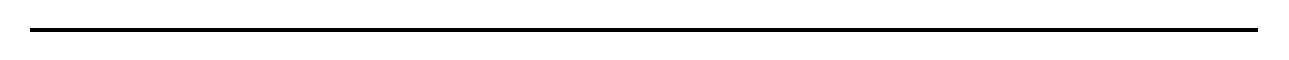
\begin{tikzpicture}
    \draw[ultra thick] (0,0) -- (15.6,0);
\end{tikzpicture}

\textbf{调和函数},$\{e^{imx}\}$

微分方程:
\[\dv[2]{f}{x}+m^2f=0\]

正交化:在$[0,2π]$区间

归一化因子:
\[\frac{1}{\sqrt{2\pi}}\]

存在:移动

\textbf{勒让德函数},$\{P(x)\}$

微分方程:
\[\dv{x}\left[(1-x^2)\dv{f}{x}\right]+l(l+1)f=0\]

正交化:对$[-1,1]$区间的$\{x^n\}$

归一化因子:
\[\sqrt{\frac{2l+1}{2}}\]

母函数:
\[\frac{1}{\sqrt{1-2xt+t^2}}=\sum_nP_n(x)t^n\]

存在:角运动。

联属勒让德函数,$\{P_l^m(x)\}$

微分方程:
\[\dv{x}\left[(1+x^2)\dv{f}{x}\right]+\left[l(l+1)-\frac{m^2}{1-x^2}\right]f=0\]

正交化:相同$m$,不同$l$,在区间$[-1,1]$

归一化因子:
\[\sqrt{\frac{(2l+1)(l-m)!}{2(l+m)!}}\]

存在:角运动

\textbf{拉基尔函数},$\{L_n(x)\}$

微分方程:
\[x\dv[2]{f}{x}+\dv{f}{x}-\left(\frac{1}{2}+\frac{x}{4}+n\right)f=0\]

正交化:对$[0,+\infty]$区间的$\{e^{-\frac{x}{2}}x^n\}$

归一化因子:
\[\frac{1}{n!}\]

母函数:
\[\frac{1}{1-t}e^{-\frac{xt}{1-t}}=\sum_nL_n(x)t^n\]

存在:径向运动

\textbf{厄米函数},$\{H_n(x)\}$

微分方程:
\[\dv[2]{f}{x}-2x\dv{f}{x}+2nf=0\]

正交化:对$(-\infty,+\infty)$区间的$\{e^{-\frac{x^2}{2}}x^n\}$

归一化因子:
\[\left(\frac{1}{\pi}\right)^{\frac{1}{4}}\frac{1}{\sqrt{2^nn!}}\]

母函数:
\[e^{2xt-t^2}=\frac{1}{n!}\sum_nH_n(x)t^n\]

存在:谐振子

\begin{problemset}
    \item 证明函数组$\{\sin mx,\cos nx\}$在m和n是正整数时在区间$[-\pi,\pi]$正交。
    \item 将下列函数按偶,奇,或非偶非奇分类,若函数既非偶又非奇,则将以函教分解成偶函数和奇函数之和。
    \[(a) \ x^2; \ (b) \ x^3; \ (c) \ x\sin x; \ (d) \ x^3\cos nx(n \in \mathbb{N_+}); \ (e) \ x^4; \ (f) \ \ln\left(\frac{1+x}{1-x}\right); \ (g) \ e^x; \ (h) \ e^{ix}\]
    \item 证明函数组$\{\sin mx\}$,$\{\cos nx\}$在区间$[0,\pi]$正交。求这些函数在区间的范数。计算用这些函数组展开的展开系数。
    \item 将函数$x-x^2$在区间$[-\pi,\pi]$\footnote{应该是$[0,\pi]$}展开,在区间$[0,\pi]$展成正弦级数,在区间$[0,\pi]$展成余弦级数。哪个展开式在$[0,\pi]$区间收敛的最快?
    \item 将函数$\sin^2x$在区间$[0,\pi]$展成正弦级数和余弦级数。哪个展开式收敛的最快?将结果与题4比较。
    \item 应用题4和题5的结果以及展开定理,计算在$[0,π]$的内积$\bra*{\sin x}\ket*{x-x^2}$。
    \item 证明函数组$\{e^{imx}\}$在区间$[0,2π]$正交。求此函数组的范数。计算用此函数组展开的展开系数。将这些系数与通常用富里叶级数展开的展开系数比较。
    \item “方波"是用在$0<x<\pi:f(x)=a,-\pi<x<0:f(x)=-a$定义的。对方波作富里叶级数展开。
    \item “三角波”是用在$-π≤x≤0:f(x)=x+π,0≤x≤π:f(x)=π-x$定义的。对三角波作富里叶级数展开。
    \item 证明函数组$\{exp(\frac{2ni\pi x}{b-a})\}$在区间$[a,b]$正交。
    \item 在零附近的泰勒级数是$x$的幂的展开式。泰勒级数是用正交函数展开的吗?证明各种正交归一函数组如何由用于泰勒级数的$x$的幂函数造出来的。
    \item 函数组$\{\sin^nx\}(n=0,1,2,\cdots)$不是正交归一函数组。 证明在$[-\pi,\pi]$用这组函数造的正交归一函数组就是题1的函数组。
    \item 用微分方程(方程2-110)证明联属勒让德函数事实上正如所述是正交的。
    \item 验证拉基尔多项式的正交化正如特殊函数表所列;验证其归一化因子。
    \item 验证厄米多项式的归一化因子正如特殊函数表所列。
    \item 将函数$e^x$展成勒让德多项式,厄米多项式和拉基尔多项式,井比较其结果。注意它们的展开区间十分不同。
    \item 对施密特正交化的讨论因展开区间的选择而有所不同。用一些尝试性例子说明改变展开区间对正交函数的影响是什么。
    \item 在光谱学中“选择定则”规定了哪些能级间的跃迁是允许的。对于
    “电偶级跃迁”光谱吸收的强度与称为跃迁偶级矩$\abs*{\bra*{\Psi_1}x\ket*{\Psi_2}}^2$成比例。
    计算谐振子的下列跃迁的跃迁偶极矩$(\Psi_n(x)=e^{-\frac{x^2}{2}}H_n(x))$,
    \[
    \begin{array}{ll}
        \Psi_1 \rightarrow \Psi_2 & \Psi_2 \rightarrow \Psi_3 \\
        \Psi_1 \rightarrow \Psi_3 & \Psi_2 \rightarrow \Psi_4 \\
        \Psi_1 \rightarrow \Psi_4
    \end{array}    
    \]
    你是否见到有什么花样出现?你能否列出并证明谐振子的一般选择定则?
\end{problemset}